
	\subsection{Circuito sin etapa de potencia}
		A continuación se exponen las mediciones realizadas los días \texttt{4/12/2018} y \texttt{5/12/2018} donde se valida el funcionamiento de la primer y segunda etapa del circuito. Para realizar las mismas, se desconectan las conexiones del multiplicador de $V_{BE}$ con los transistores de salida; también se conecta la realimentación global a la salida del VAS dado que el mismo provee la misma tensión que la salida del circuito completo. Sin embargo para emular la conexión de la tercer etapa, se conecta una resistencia de valor comercial \SI{39}{\kilo\ohm} que es aproximadamente igual a la carga que presenta la reflexión de $R_L$ (con valor teórico de \SI{36}{\kilo\ohm}).\\
		\indent Con dichas consideraciones se procede a realizar las mediciones.
		\graficarEPS{0.6}{banco_med}{Diagrama del circuito para mediciones sin etapa de potencia.}{fig:banco_med}

		\subsubsection{Polarización}
		
		Las mediciones de polarización se realizaron con el multímetro \emph{UT30D} cortocircuitando la entrada y se exponen en la Figura \ref{fig:51218_pol}. Cabe destacar que las mediciones en color rojo corresponden a tensiones con respecto a masa y aquellas en color azul, diferencia de potencial.
		
		\begin{figure}[h!]
			\centering
			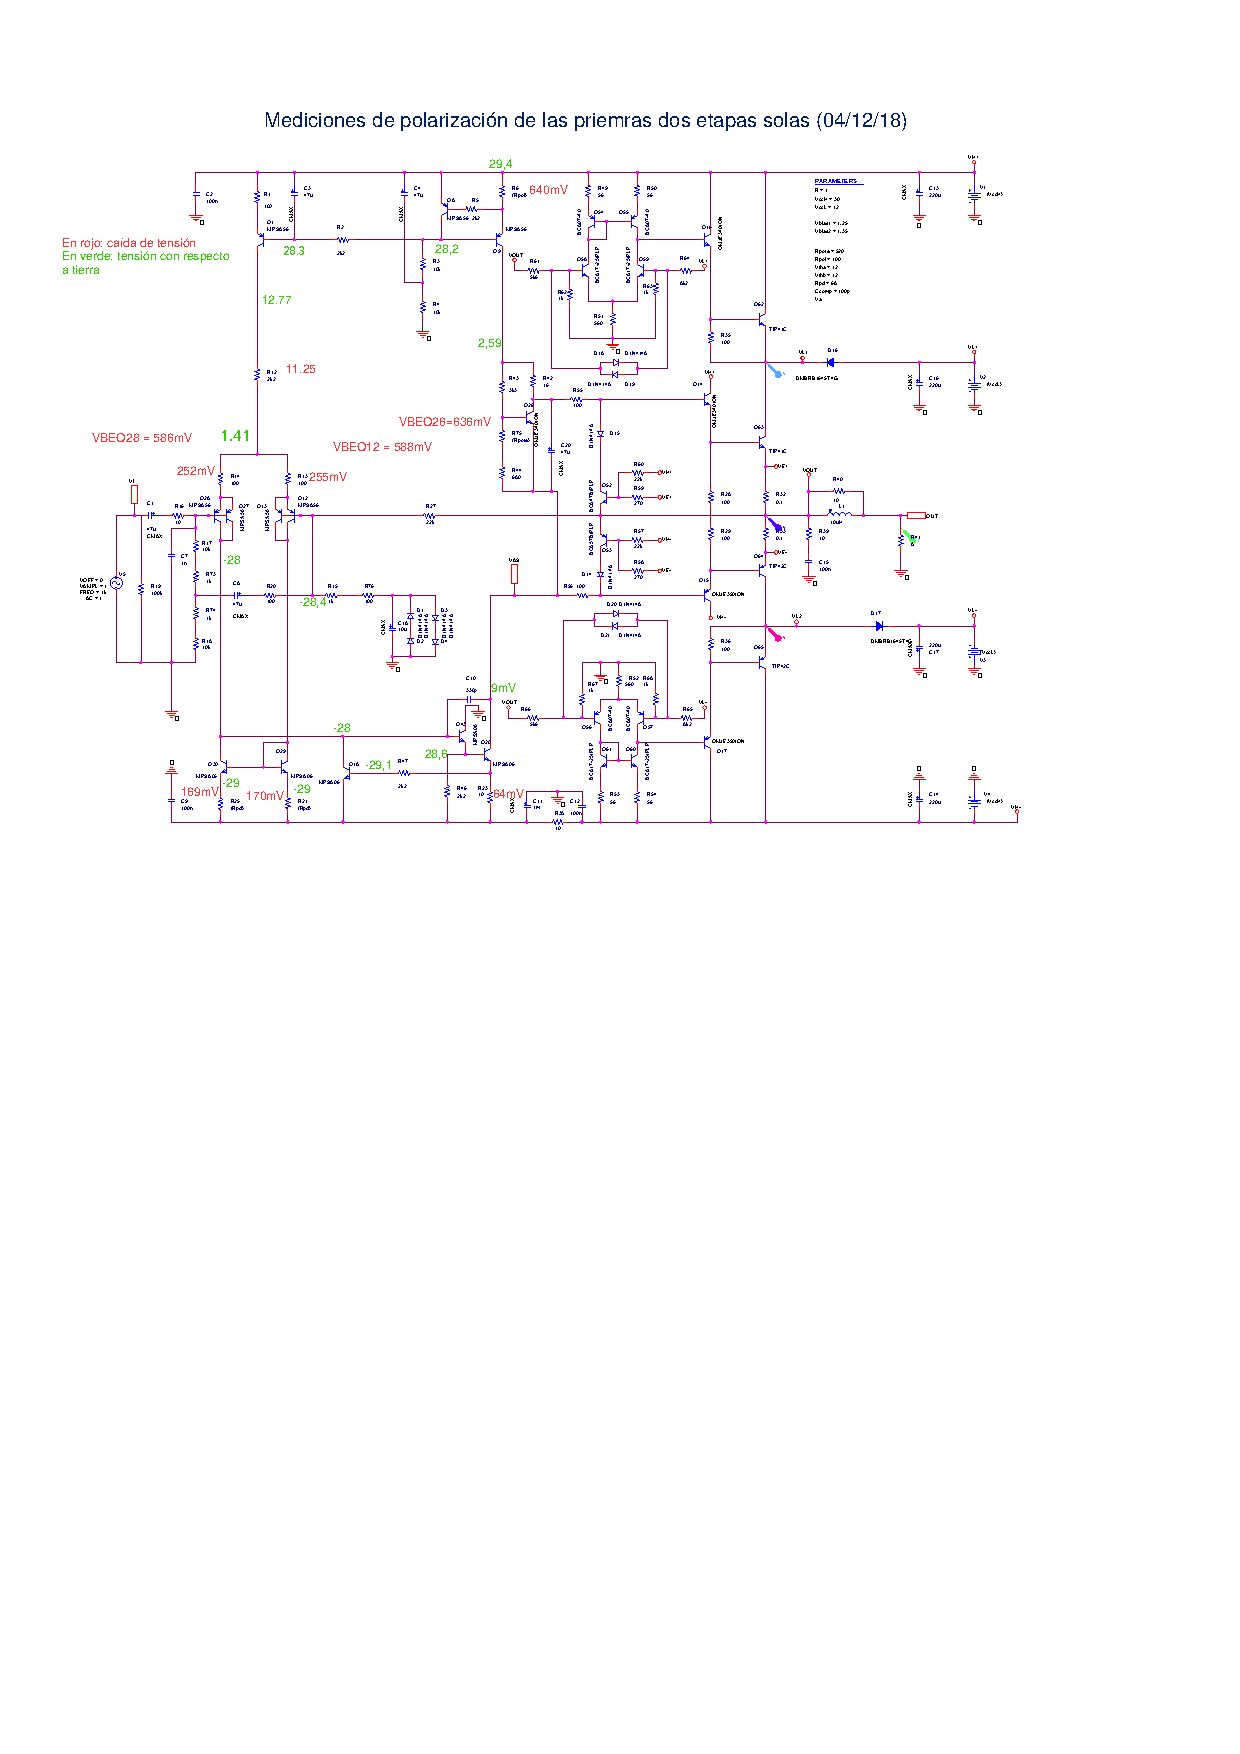
\includegraphics[angle=-90, scale=0.6]{./Mediciones/1_mediciones.pdf}
			\caption{Mediciones de polarización del día \texttt{4/12/2018}.}
			\label{fig:51218_pol}
		\end{figure}
		
		%\begin{figure}[h!]
		%	\centering
		%	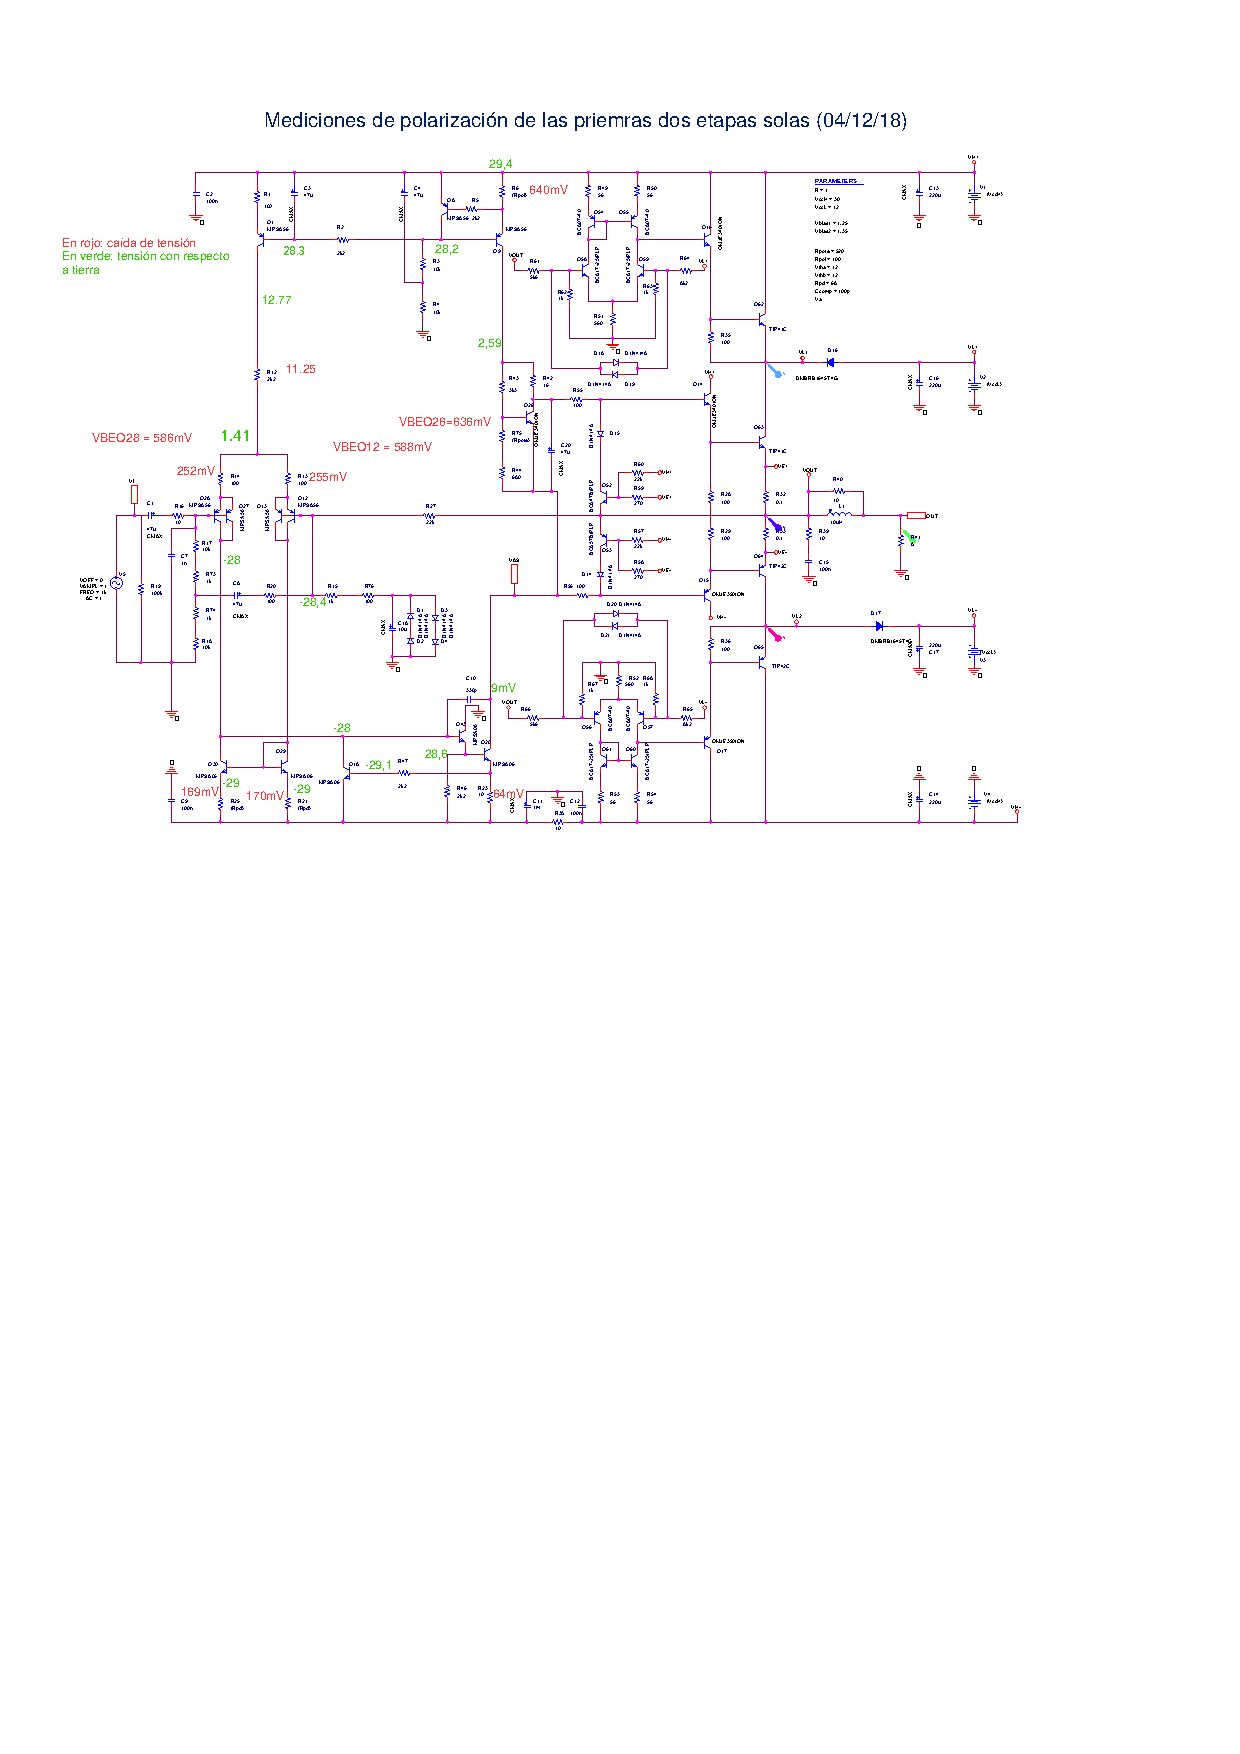
\includegraphics[width=0.8\textwidth, trim = 2cm 14cm 4cm 1cm]{./Mediciones/1_mediciones.pdf}
		%	\caption{Mediciones de polarización del día \texttt{4/12/2018}.}
		%	\label{fig:51218_pol}
		%\end{figure}

		\subsubsection{Impedancia de entrada}
			
		\begin{figure}[ H]
			\centering
			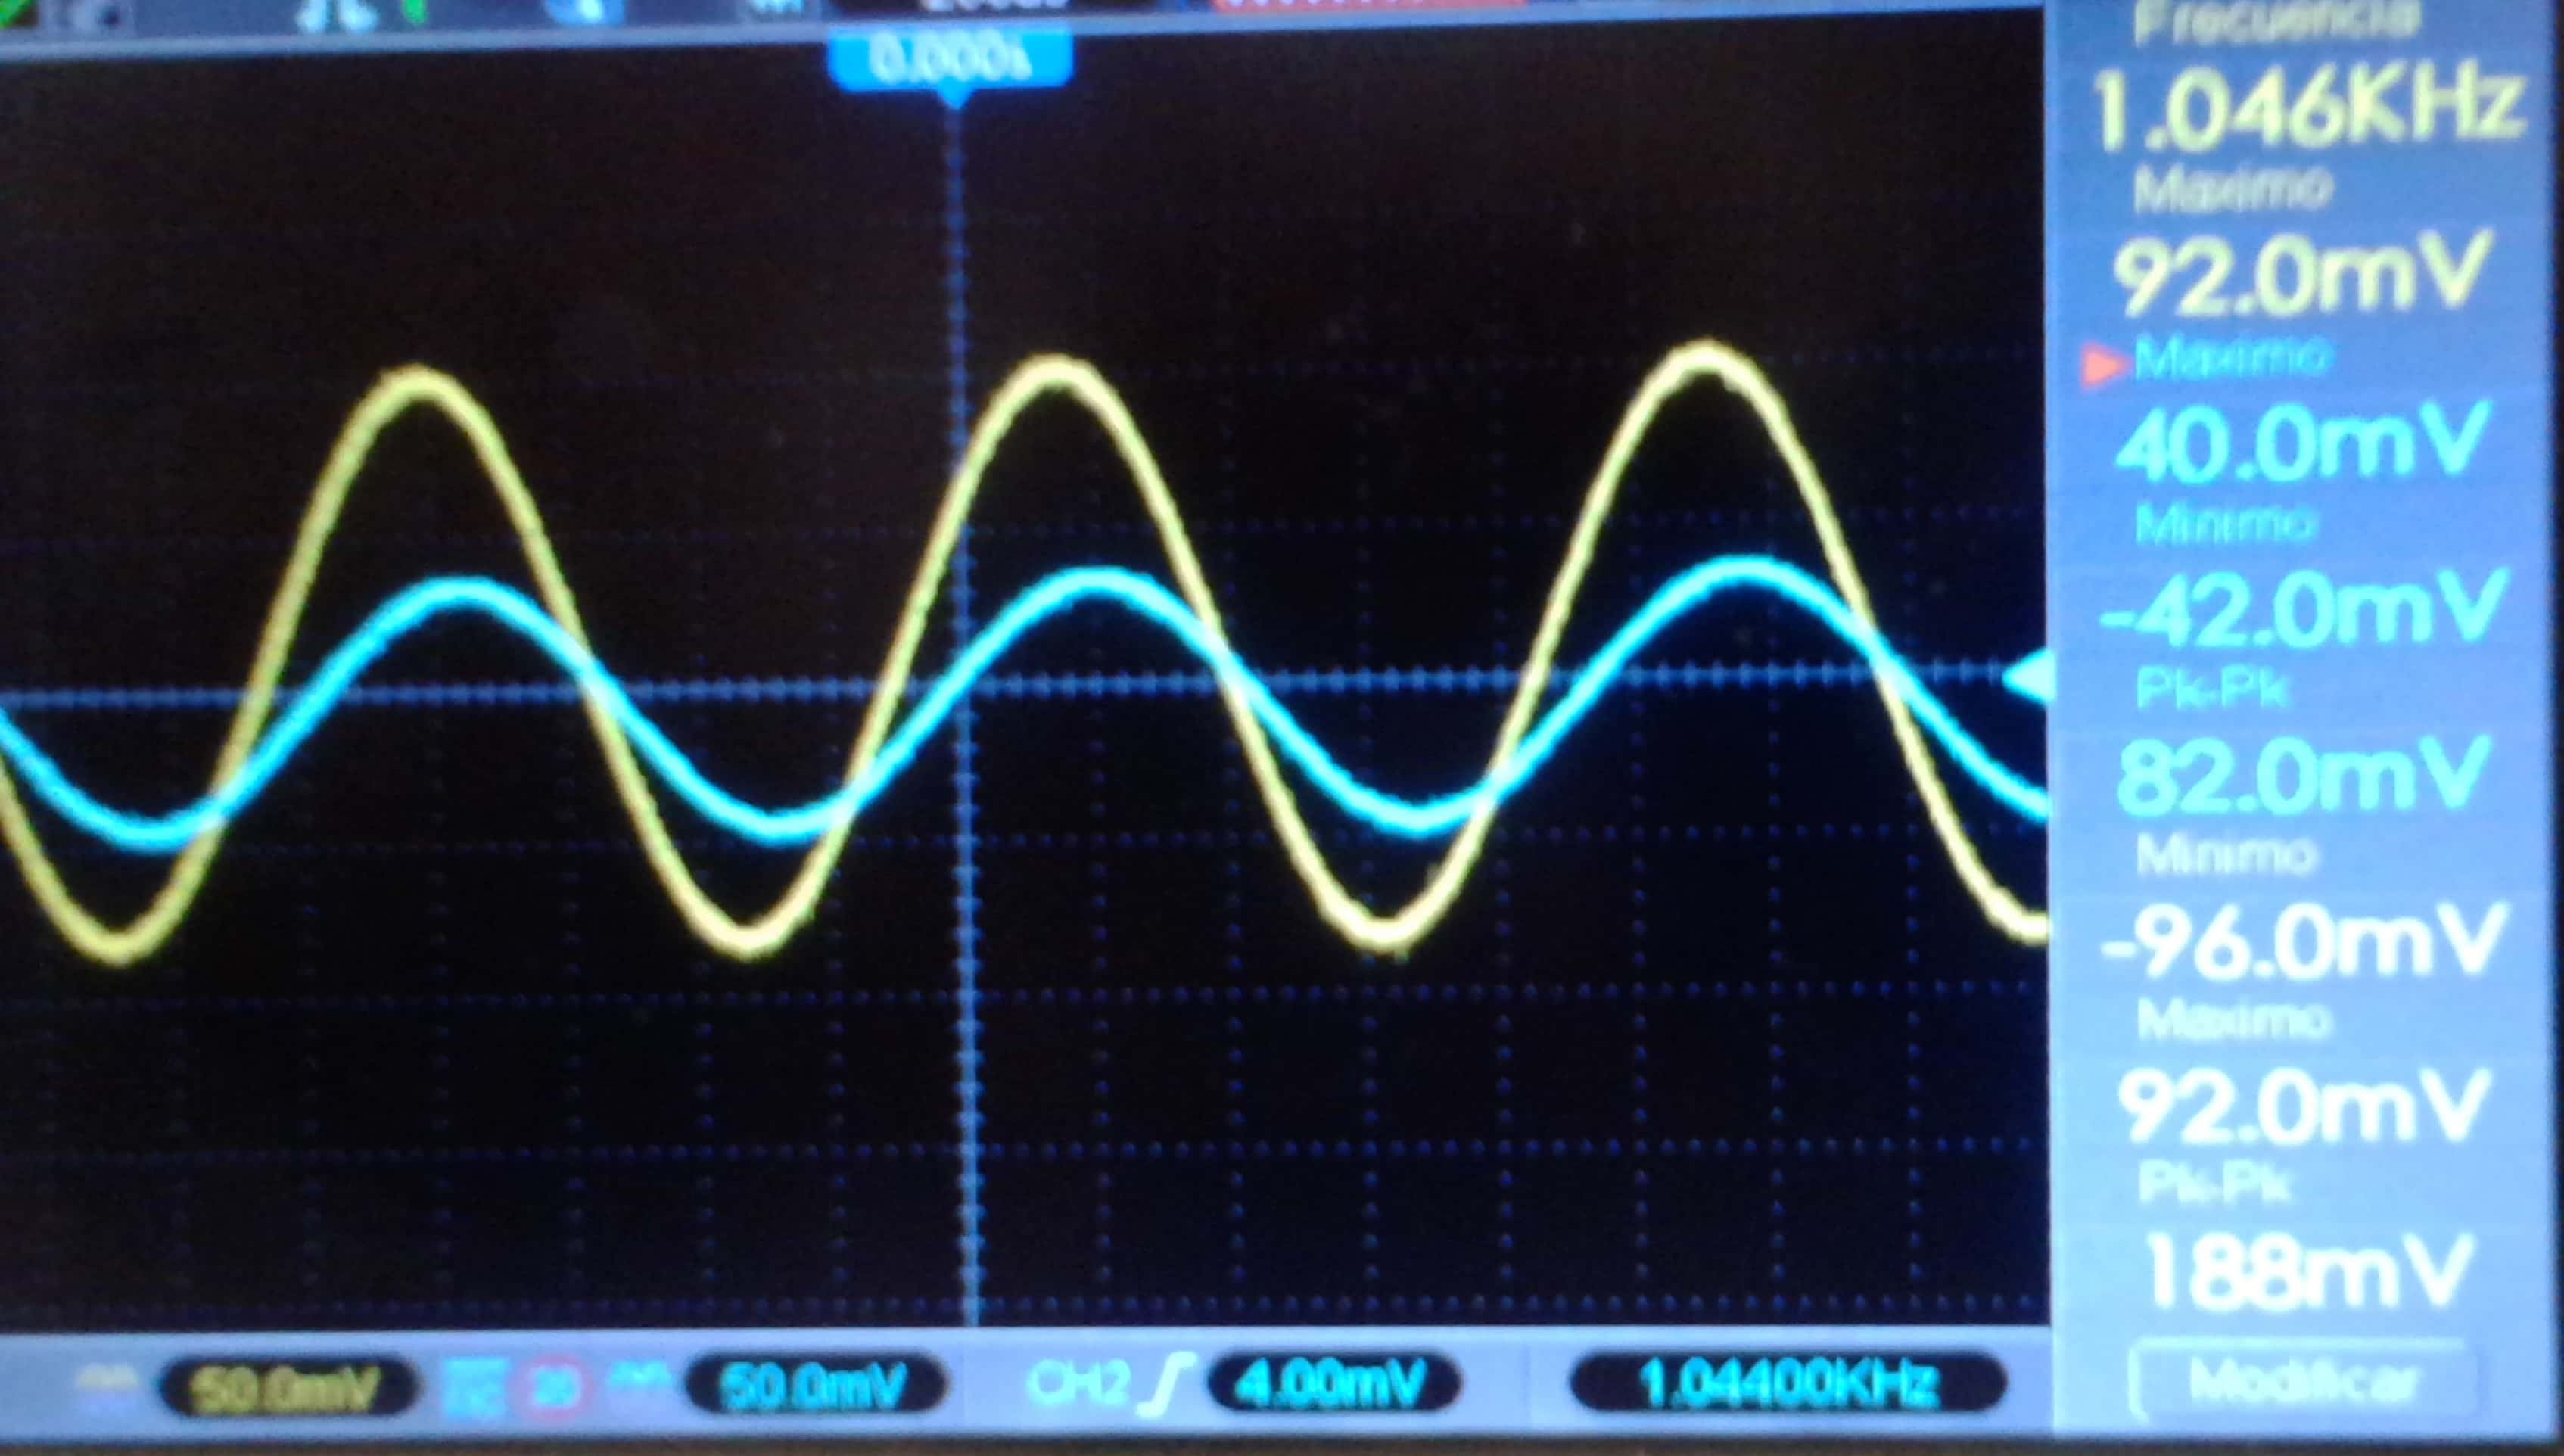
\includegraphics[width=0.8\textwidth]{./Mediciones/Rin_1k.jpg}
			\caption{Medición de las tensiones de generador de prueba y el nodo de entrada.}
			\label{fig:rin_med}
		\end{figure}

		\begin{figure}[ H]
			\centering
			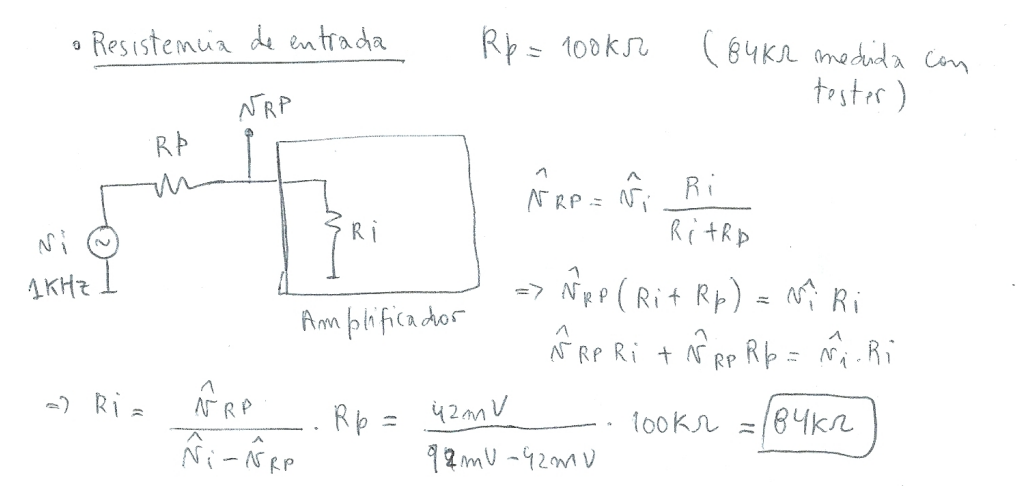
\includegraphics[width=1.0\textwidth]{./Mediciones/Rin_1k_calculo.png}
			\caption{Análisis detallado de la medición de $R_{in}$.}
			\label{fig:analisis_rin_med}
		\end{figure}

		Para la medición de resistencia de entrada, se inyecta una señal conocida al circuito con resistencia serie lo más similar posible a la resistencia de entrada propia del amplificador. La tensión medida está relacionada con el divisor resistivo generado entre $R_{p}$ y $R_{in}$ de forma tal que se puede hallar indirectamente dicha resistencia. La medición se expone en la Figura \ref{fig:rin_med} y en la Figura \ref{fig:analisis_rin_med} se realiza la explicación y cálculo de dicha resistencia resultando $\boxed{R_{in}=\SI{84}{\kilo\ohm}}$.\\

		Del mismo modo se realizó la medición de $R_{in}$ para frecuencia de \SI{10}{\kHz} resultando en:
		\begin{equation*}
			R_{in}(@\SI{10}{\kHz})  = \frac{\SI{13.2}{\mV}}{\SI{94}{\mV} - \SI{13.2}{\mV}} \, \SI{100}{\kilo\ohm} = \boxed{\SI{16.3}{\kilo\ohm}}
		\end{equation*}
		\subsubsection{Ancho de banda de potencia}

	\graficarEPS{1.0}{Mediciones/graf_BW_pot}{Respuesta en frecuencia para tensiones de entrada $V_{pp} = \SI{1.1}{\V}$.}{fig:pot_BW_med}
		
		A través de la Figura \ref{fig:pot_BW_med} se halla la frecuencia en la cual la respuesta en frecuencia disminuya \SI{3}{\dB}. La frecuencia de corte es por tanto:
		\begin{equation*}
			\boxed{f_H \approx \SI{130}{\kHz}}
		\end{equation*}

		\subsubsection{Respuesta al escalón}
		\begin{figure}[h!]
			\centering
			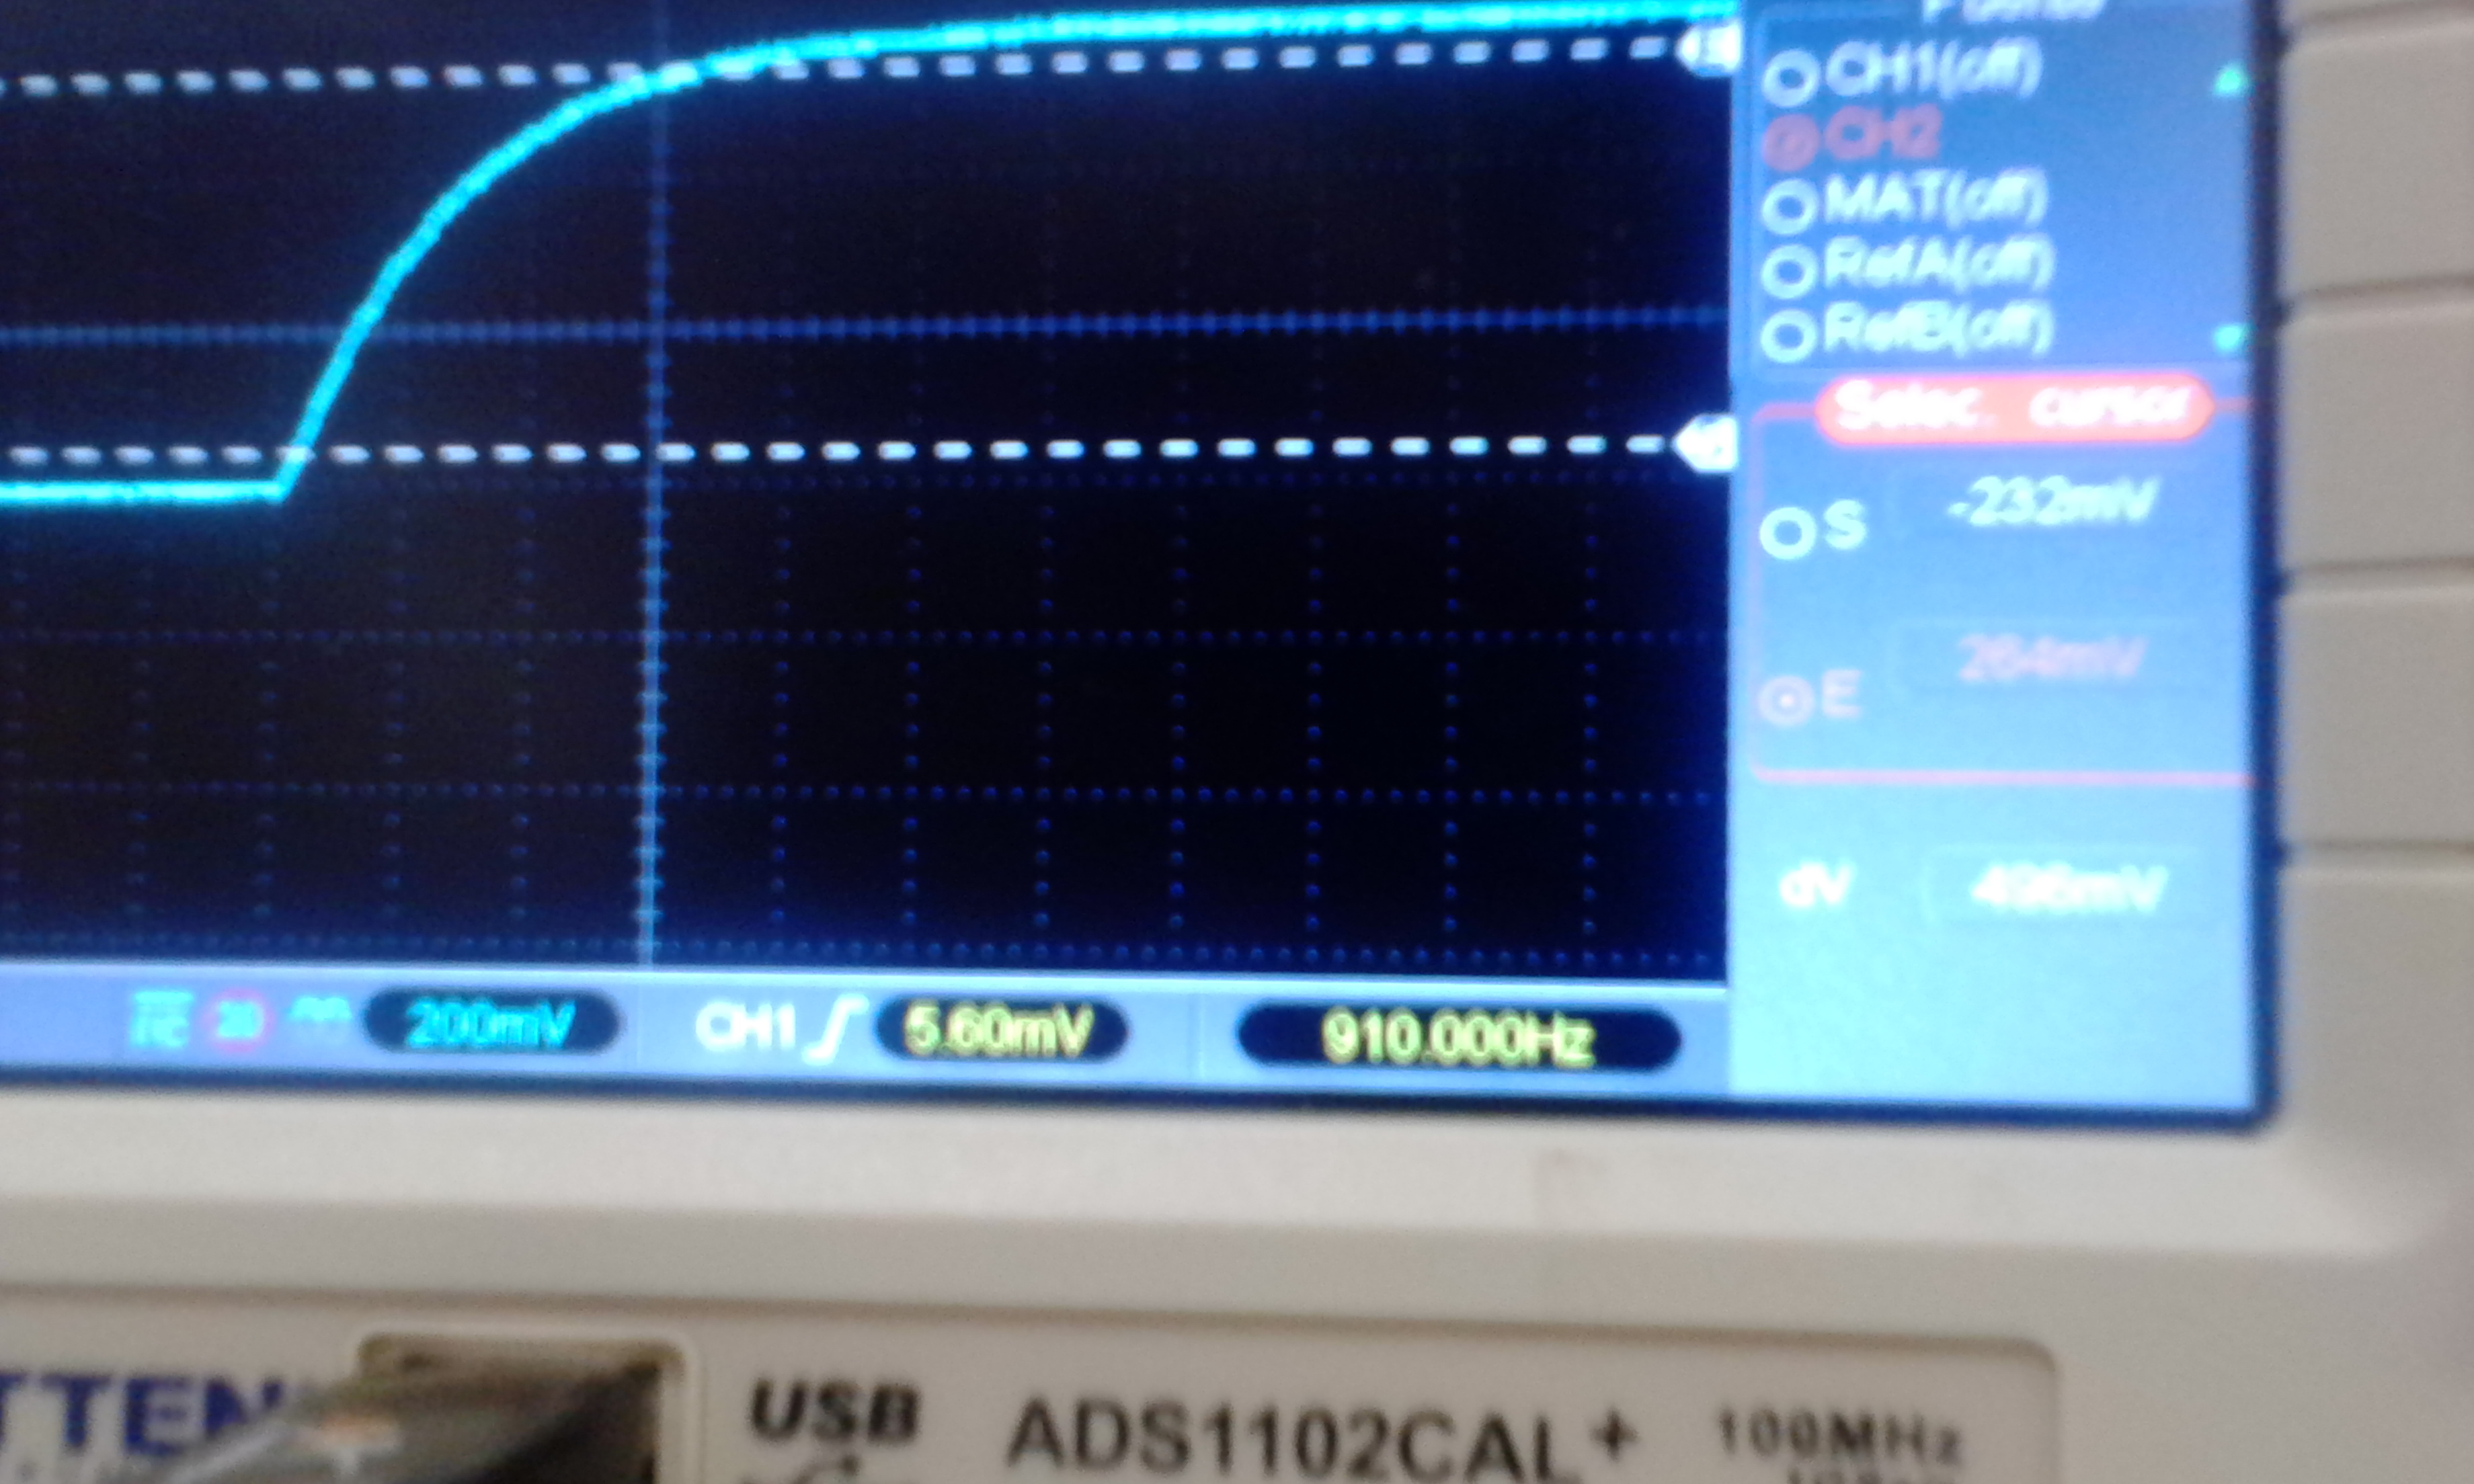
\includegraphics[width=0.8\textwidth]{./Mediciones/BW.jpg}
			\caption{Respuesta al escalón en pequeña señal.}
			\label{fig:escalon_ss}
		\end{figure}

		\begin{figure}[h!]
			\centering
			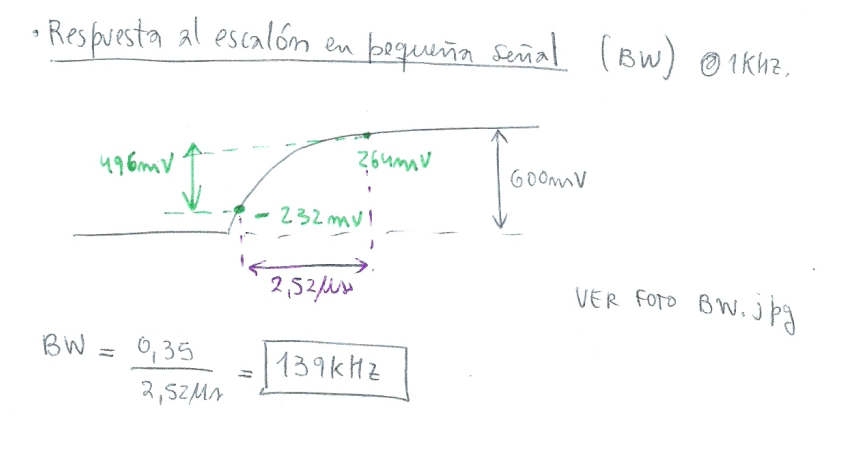
\includegraphics[width=1.0\textwidth]{./Mediciones/BW_calculo.png}
			\caption{Análisis detallado de la medición de respuesta al escalón en señal.}
			\label{fig:analisis_escalon_ss}
		\end{figure}

		Se conecta un generador a la entrada con un escalón de \SI{1}{\kHz}. La medición se expone en la Figura \ref{fig:escalon_ss} y el análisis del mismo se detalla en la Figura \ref{fig:analisis_escalon_ss} resultando en
		\begin{equation*}
			\boxed{BW = \SI{139}{\kHz}}
		\end{equation*}

		\subsubsection{\emph{Slew Rate}}
		Se realiza una medición similar a la anterior, salvo que en este caso la entrada es un escalón que va de \SI{-.6}{\V} a \SI{.6}{\V}. Así a partir de la medición de la Figura \ref{fig:sr_med} como se detallan los valores en la Figura \ref{fig:analisis_sr_med} se obtiene un \emph{Slew Rate} similar al simulado de $\boxed{SR = \SI{8}{\V\per\micro\second}}$.

		\begin{figure}[h!]
			\centering
			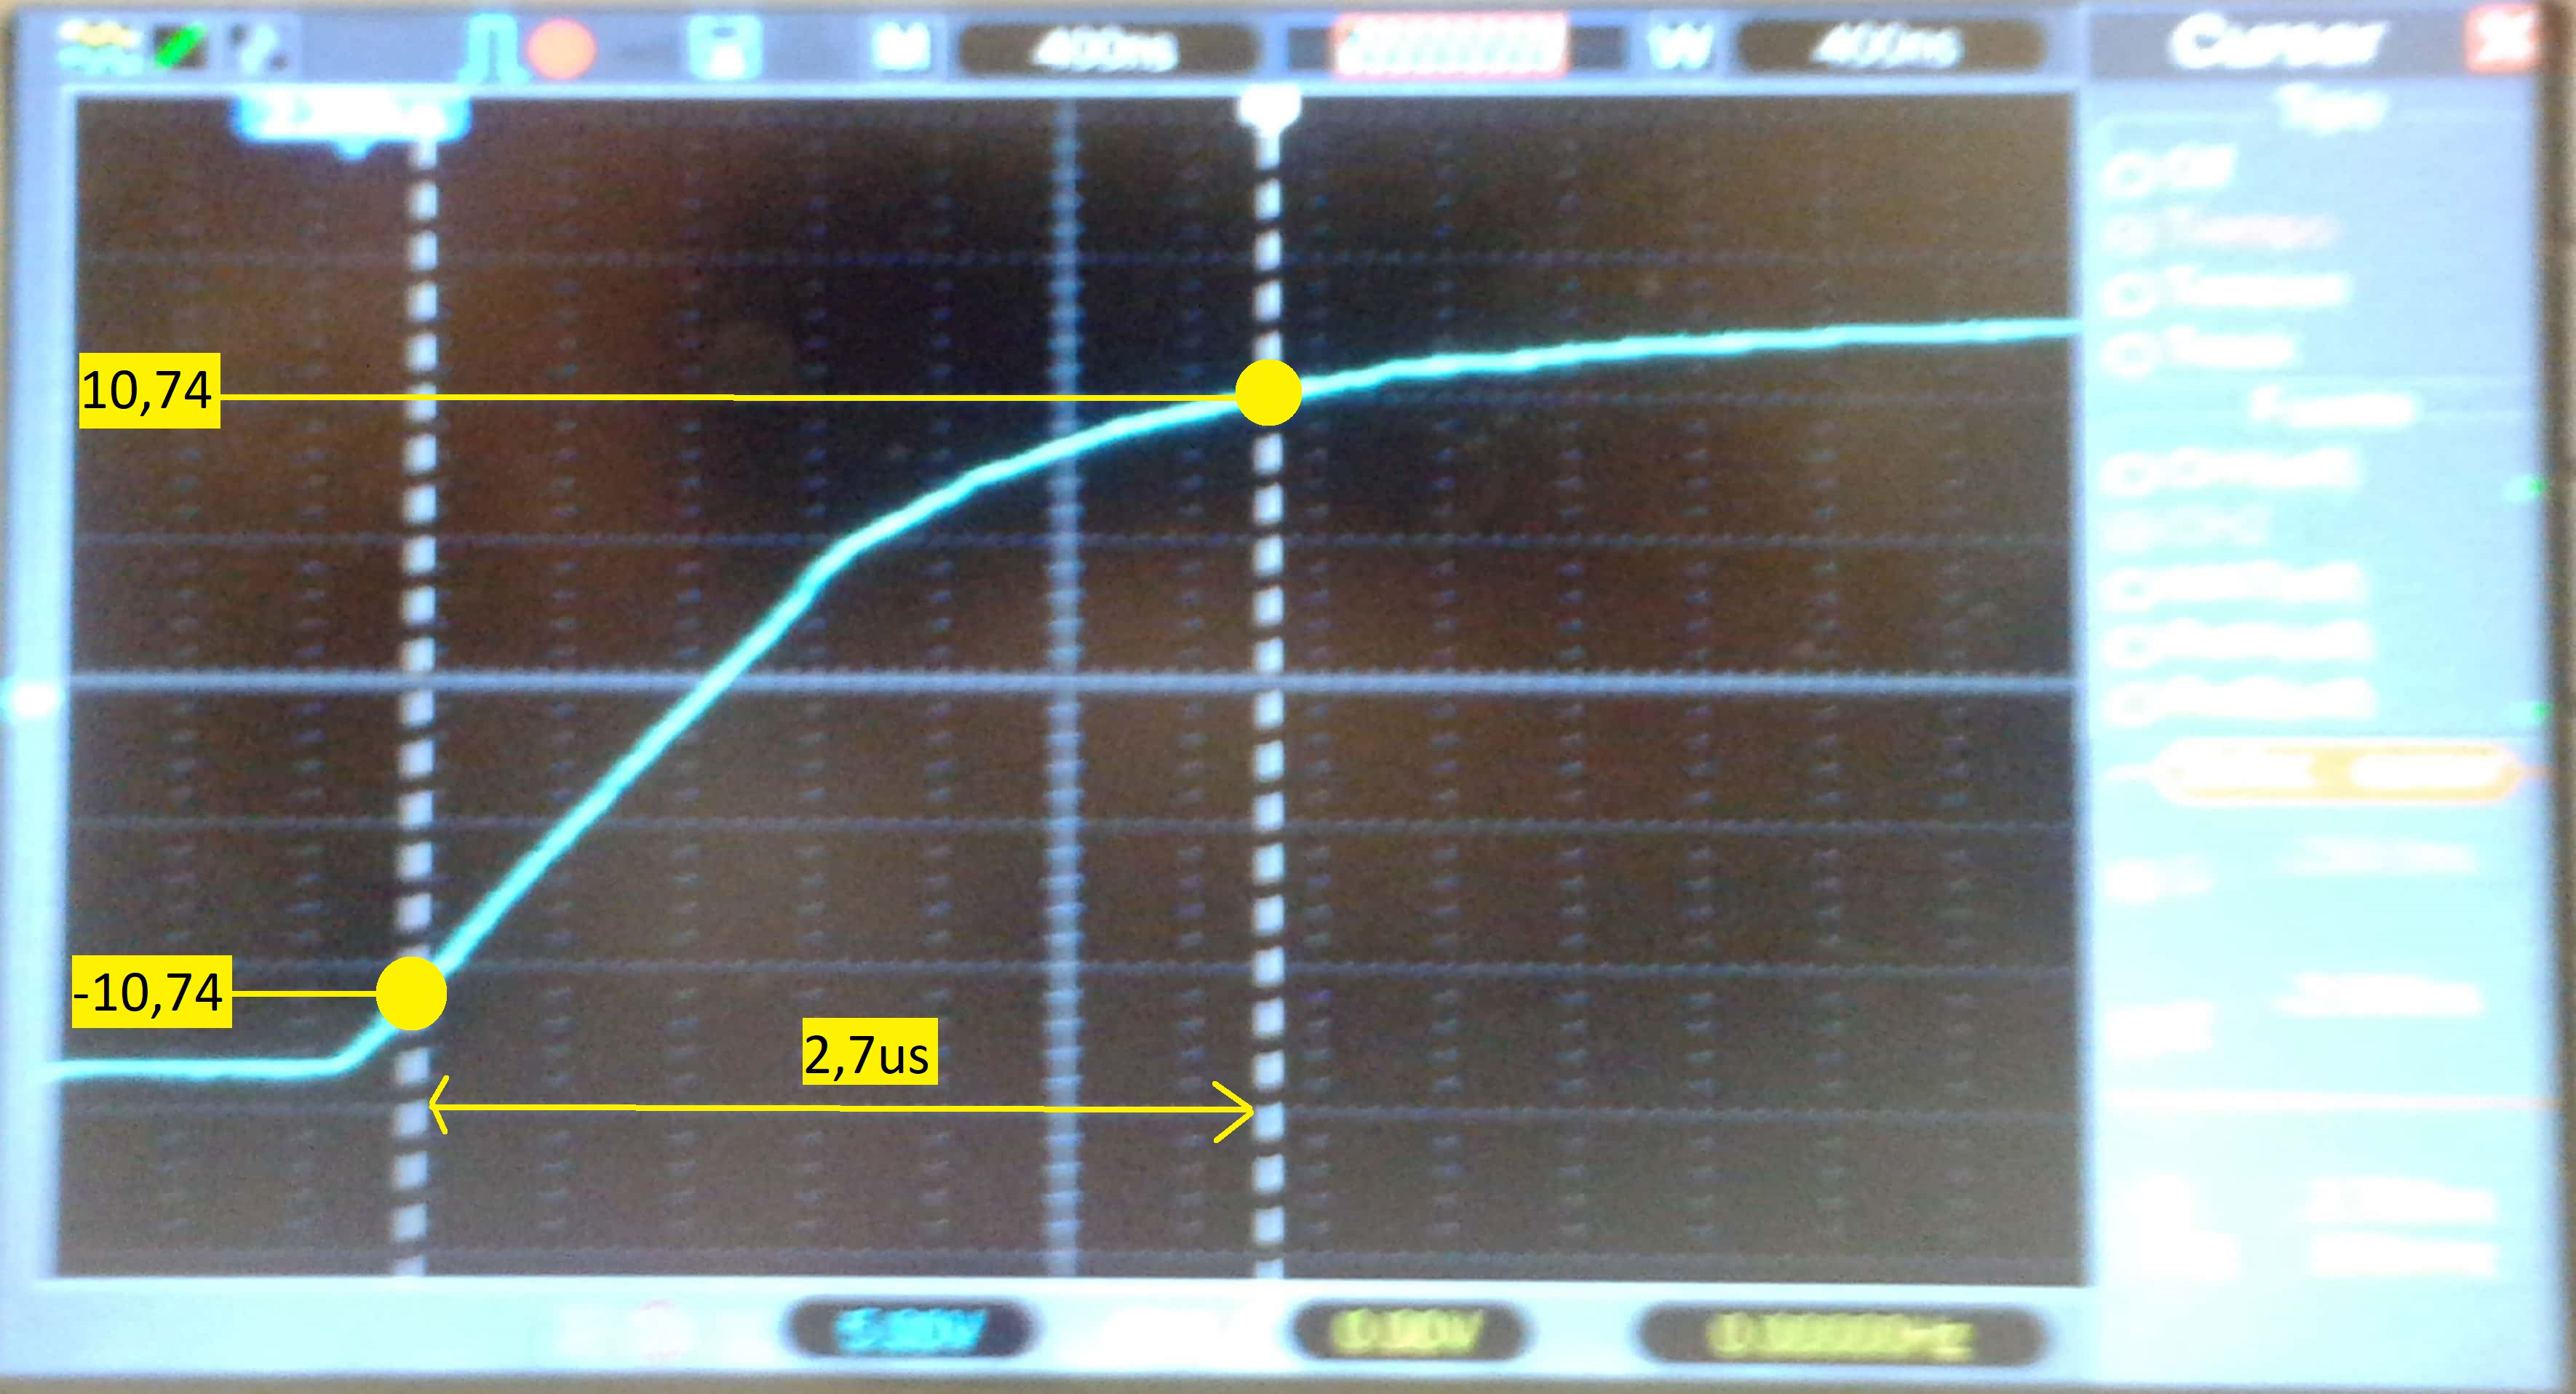
\includegraphics[width=0.8\textwidth]{./Mediciones/SR2.jpg}
			\caption{Respuesta al escalón en gran señal para hallar el \emph{Slew Rate}.}
			\label{fig:sr_med}
		\end{figure}

		\begin{figure}[h!]
			\centering
			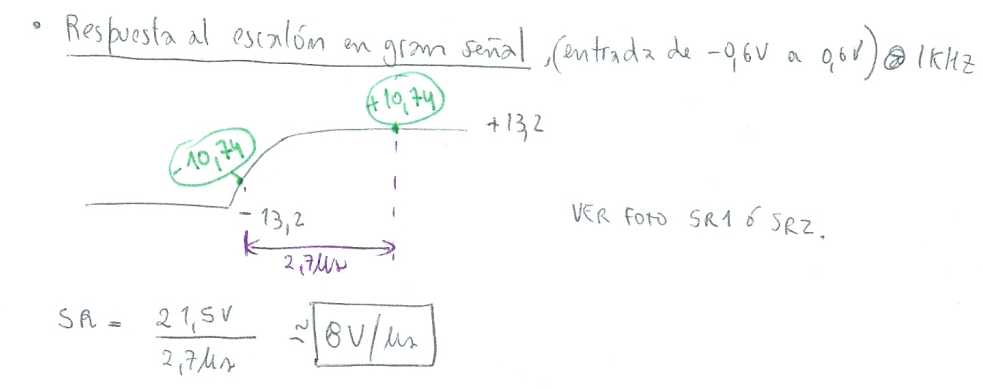
\includegraphics[width=1.0\textwidth]{./Mediciones/SR_calculo.png}
			\caption{Análisis detallado de la medición del \emph{Slew Rate}.}
			\label{fig:analisis_sr_med}
		\end{figure}

		\subsubsection{Variación de la Fuente de Alimentación}
		
		\graficarPNG{0.4}{./Mediciones/Variacion_fuente}{Mediciones de las caídas de potencial para 2 juegos de tensiones de alimentación.}{fig:var_fuente_med}
		En este caso se alimentó el circuito con $V_{CCH+}$ y $V_{CCH-}$ pero se supone que dichas fuentes no son muy buenas. Por tanto se midieron las caídas de potencial sobre las resistencias con los valores de alimentación común y con alimentaciones menores al 10\%. Los resultados y mediciones se exponen en la Figura \ref{fig:var_fuente_med} mostrando errores menores al \num{1.8}\%.


		\subsubsection{Distorsión armónica}
		
			Se realizó un análsis de \emph{FFT} del circuito ingresando con una señal de \SI{1}{\kHz}, pero no se pueden sacar conclusiones de la medición de la Figura \ref{fig:fft_med} porque el piso de ruido es muy alto y no se puede ver el efecto de los harmónicos. Para ello habría que utilizar un \emph{software} que permita ingresar señales particulares y ver el comportamiento en frecuencia del circuito ante esos estímulos.

		\graficarPNG{0.1}{./Mediciones/FFT}{Análisis del circuito por Fourier.}{fig:fft_med}

		\subsubsection{Máxima excursión de salida}
			
		Se introdujo una señal de amplitud tal que la salida no recorte. Dicha señal corresponde a una de amplitud pico a pico \SI{1.1}{\V}. A la salida se obtiene $V_{pp} = \SI{32.4}{\V}$.

		\HgraficarPNG{0.1}{./Mediciones/Maxima_excursion}{Medición de máxima excursión de salida sin recorte.}{fig:excursion_med}

		\subsection{Circuito completo}
		\graficarEPS{0.6}{banco_med_full}{Diagrama del circuito para mediciones con etapa de potencia.}{fig:banco_med_full}
		A continuación se presentan las mediciones realizadas durante la semana del \texttt{18/02/2019}. Se realizó el conexionado del circuito de modo tal que se tiene el circuito completo como se muestra en la Figura \ref{fig:banco_med_full}. 

		%\section{Cambios durante las mediciones}
			%Cortocircuitamos el inductor y la carga en su lugar posta.

			%Medicion slew rate: entramos con \SI{200}{\mV} y \SI{250}{\mV} y frecuencai \SI{1}{\kHz}.

		\subsubsection{Polarización}
			Con el fin de obtener un valor bajo de THD, se ajustó el potenciómetro del multiplicador de $V_{BE}$, obtenéndose los valores de la tabla \ref{tab.valores}.

		\subsubsection{Máxima excursión}
		Se introdujo una señal de amplitud (máxima) tal que la salida no recorte. Dicha señal corresponde a una
		de amplitud pico a pico 2.14 $V_{pp}$. A la salida se obtiene $V_{pp}$ = 50 V.

		\begin{figure}[h!]
			\centering
			\includegraphics[scale=0.1]{Mediciones/PotenciaMaxima.jpg}
			\caption{Medición de máxima excursión de salida antes del recorte.}
			\label{fig:MaxExcur}
		\end{figure}

		\subsubsection{Variación de la fuente}
		Al variar la fuente de alimentación entre -25 y 33 V, se miden los distintos puntos de polarizacion, tal que las corrientes de polarización no varien mas de un 10 por ciento.
		\begin{table}[]
		\begin{tabular}{|l|l|l|l|l|l|l|l|l|l|l|}
		\hline
		Vcc{[}V{]} & -Vcc{[}V{]} & A{[}V{]} & B{[}V{]} & C{[}V{]} & D{[}V{]} & E{[}V{]} & F{[}mV{]} & G{[}mV{]} & H{[}V{]} & I{[}mV{]} \\ \hline
		30.11      & 30          & 12.36    & 1.369    & -29.07   & 1.31     & -1.275   & 27.3      & 11.8      & 29.43    & 10.6      \\ \hline
		31.24      & 30.99       & 12.39    & 1.364    & -29.68   & 1.308    & -1.271   & 25.5      & 7.6       & 28.12    & 10.5      \\ \hline
		32.71      & 32.56       & 12.4     & 1.362    & -31.24   & 1.310    & -1.275   & 27.2      & 10.6      & 32.06    & 10.6      \\ \hline
		24.98      & 25          & 12.06    & 1.358    & -23.69   & 1.309    & -1.270   & 24.6      & 6.3       & 24.37    & 9.9       \\ \hline
		26.99      & 27.02       & 12.18    & 1.363    & -25.7    & 1.309    & 1.27     & 26.1      & 9.6       & 26.37    & 10.3      \\ \hline
		28.39      & 28.18       & 12.25    & 1.363    & -26.86   & 1.311    & -1.27    & 27.1      & 10.2      & 27.75    & 9.2       \\ \hline
		29.21      & 29.13       & 12.29    & 1.363    & -27.82   & 1.311    & -1.275   & 26.2      & 10.4      & 28.58    & 9.3       \\ \hline
		\end{tabular}
		\label{tab.valores}
		\end{table}

		En el esquema \ref{fig:esq_med} se marcan los puntos correspondientes a las mediciones de polarización de la tabla \ref{tab.valores}.

		\begin{figure}[H]
			\centering
			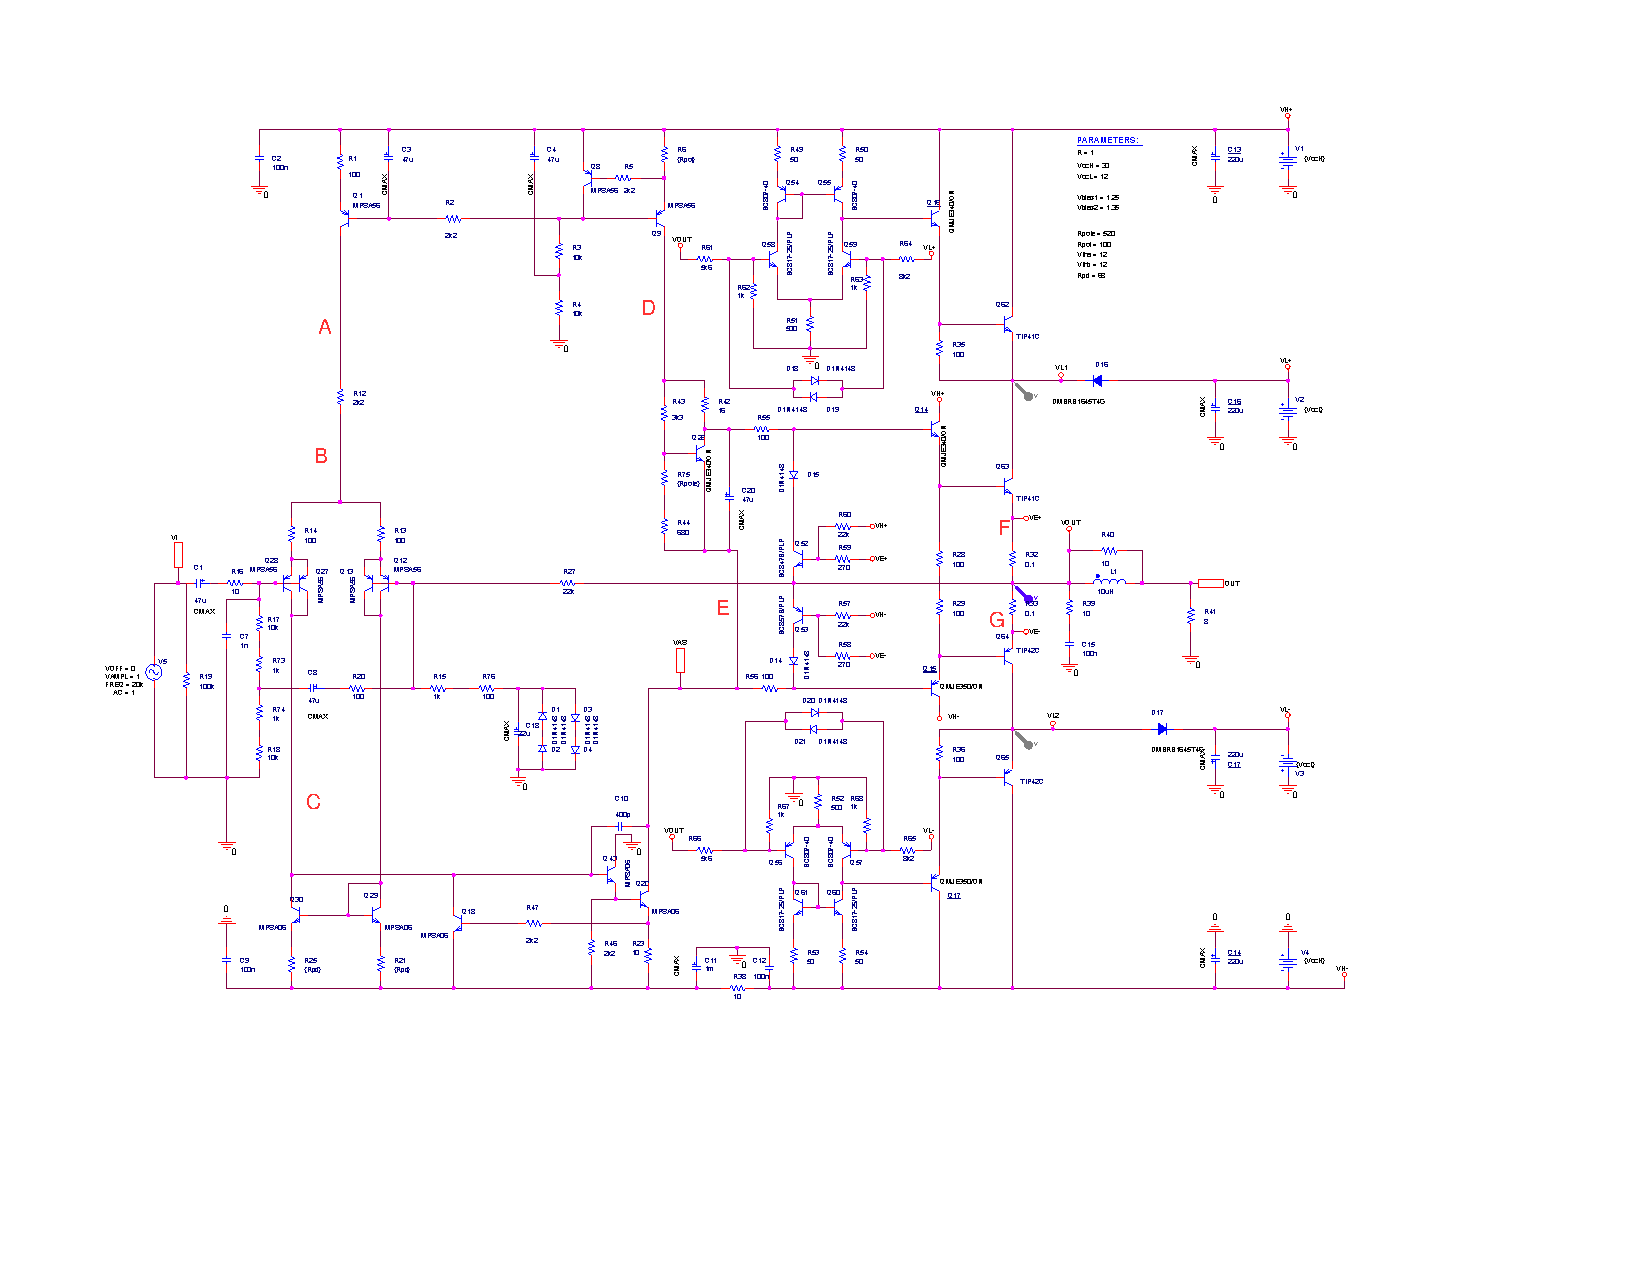
\includegraphics[scale=0.6]{./Figuras/esquema_puntos.pdf}
			\caption{Puntos de medición.}
			\label{fig:esq_med}
		\end{figure}

		\Gus{hay que calcular las corrientes y sus variaciones}
		\subsubsection{Distorsión total armónica}

		El banco de medición para la distorsión total armónica se muestra en la figura \ref{fig:thd_bco}. Los valores se obtuvieron mediante el software \textit{SpectraPlus}. Se utilizó la placa de audio de la PC para generar la señal, ya que un generador de laboratorio presenta un valor elevado de \texttt{THD}. Asimismo es necesario utilizar un atenuador resistivo debido a que la PC no admite como entrada un valor mayor a 1Vrms. 

		\begin{figure}[h!]
			\centering
			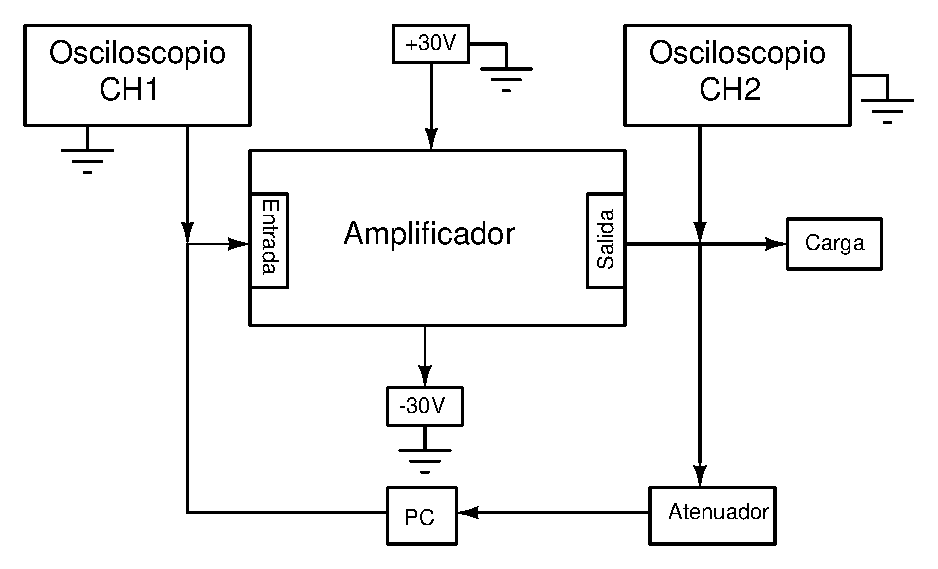
\includegraphics[scale=0.6]{./Figuras/banco_thd.eps}
			\caption{Banco de medición de \texttt{THD}.}
			\label{fig:thd_bco}
		\end{figure}

		\begin{figure}[H]
			\centering
			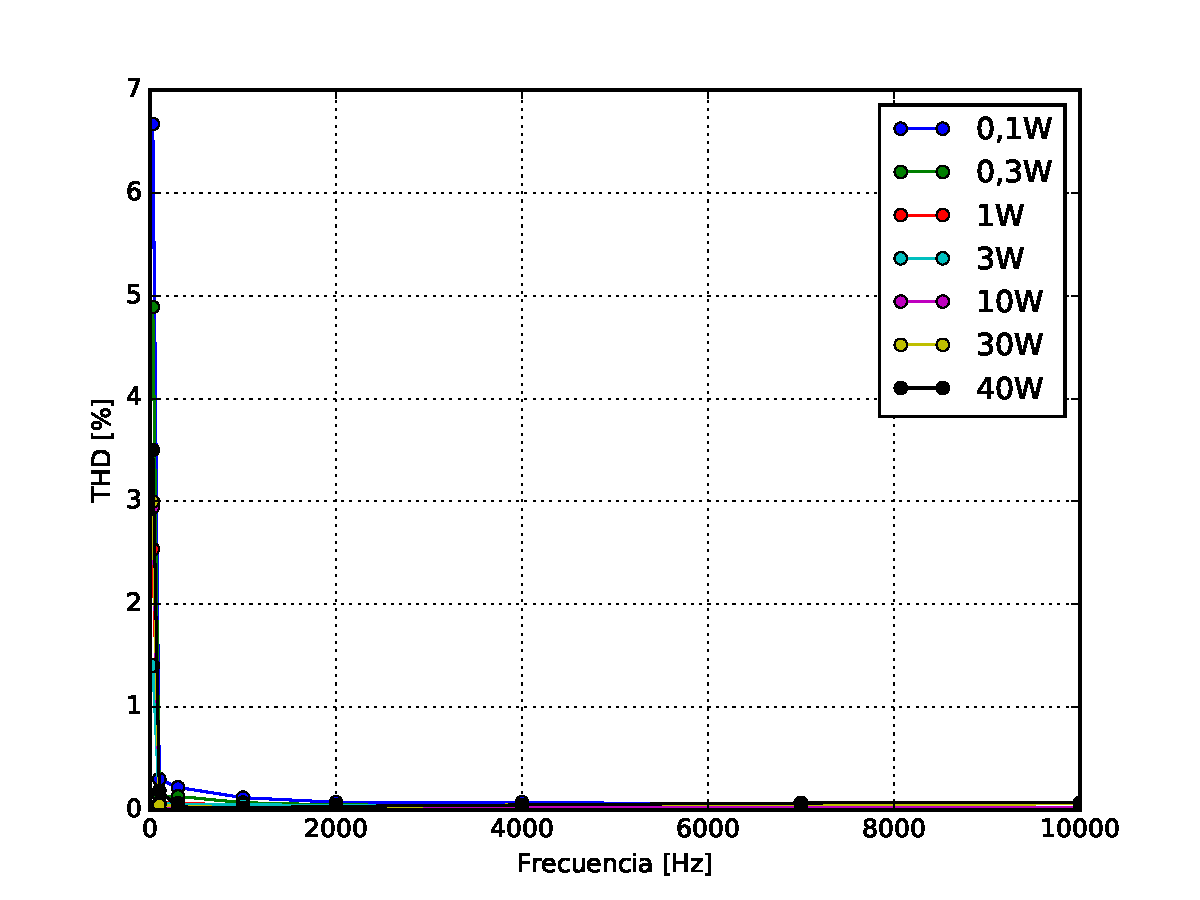
\includegraphics[scale=0.6]{./Figuras/thd.pdf}
			\caption{THD en función de la frecuencia.}
			\label{fig:thd}
		\end{figure}

		\begin{figure}[H]
			\centering
			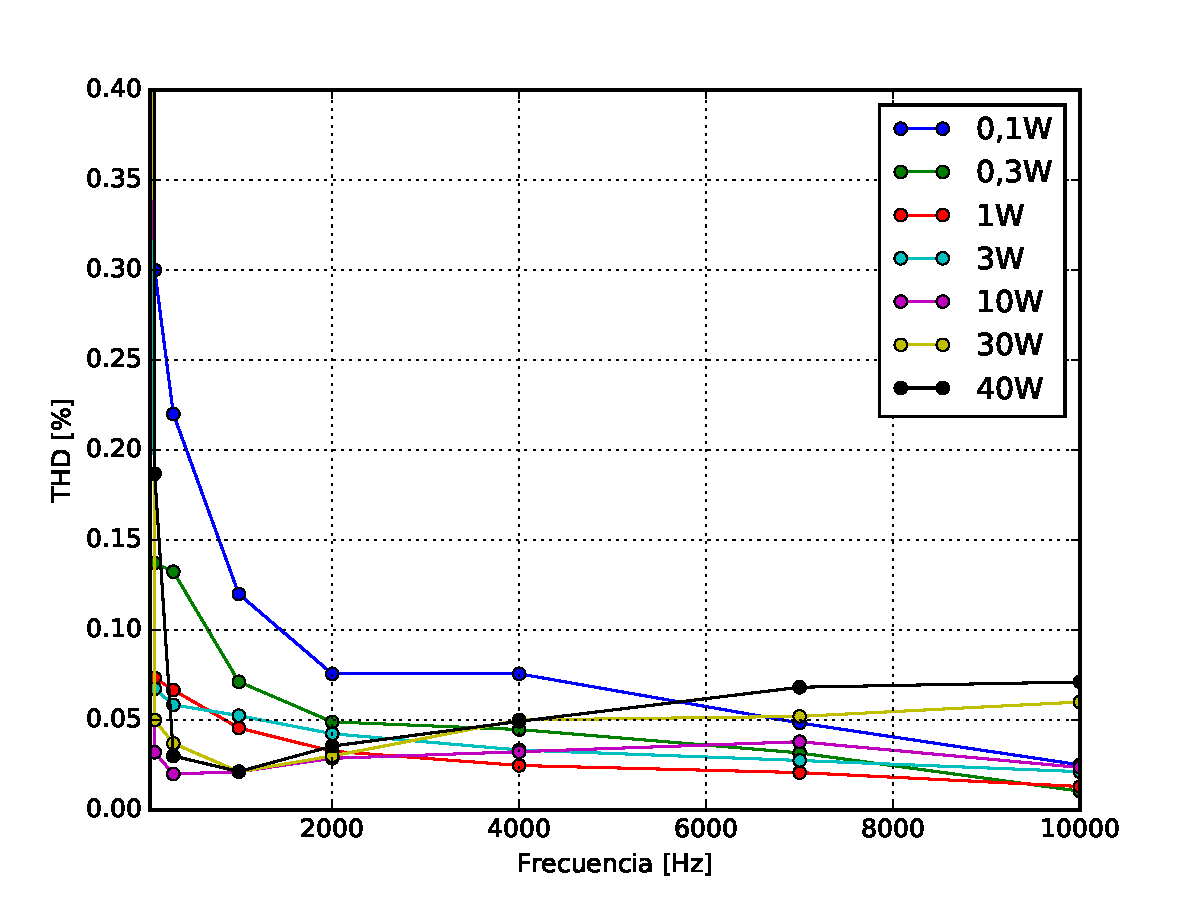
\includegraphics[scale=0.6]{./Figuras/thd_zoom.pdf}
			\caption{THD en función de la potencia.}
		\end{figure}



%		\subsubsection{Compensación}
%
%		\subsubsection{Respuesta en frecuencia}
%
		\subsubsection{Impedancia de salida}
%
%		\subsubsection{Margen de fase}
%
		\subsubsection{Distorsión por intermodulación}

		De manera análoga a la simulación, se calculó la IMD mediante el \textit{software SpectraPlus} con el mismo banco de medición que la Figura \ref{fig:thd_bco}. Las mediciones se realizaron a \SI{5}{\kilo\hertz} para las potencias \SI{0.1}{\watt}, \SI{1}{\watt}, \SI{10}{\watt}

			\begin{table}[H]
				\centering
				\begin{tabular}{cc}
				\toprule
				Potencia [W] & IMD [\%]\\
				\midrule
				0,1 & 0.0593 \\
				1 & 0,0254 \\
				10 & 0,0127 \\
				40 & 0,0253 \\
				\bottomrule
				\end{tabular}
			\end{table}
			%\Flor{Valores para 100 y 5kHz como la simulación. Tambien está 60 7k hecha}



		\subsubsection{Slew-Rate y Ancho de banda de Potencia}
		Se mide a maxima potencia a $1Khz$ y se calcula la pendiente a la salida que se genera por la respuesta al escalón.
		\Gus{Foto}

		\begin{equation*}
			SR  = \frac{\varDelta v}{\varDelta t} = 7.4 \frac{V}{us}
		\end{equation*}

		\subsubsection{Eficiencia}

		\subsection{Respuesta en frecuencia}

		\begin{figure}[H]
			\centering
			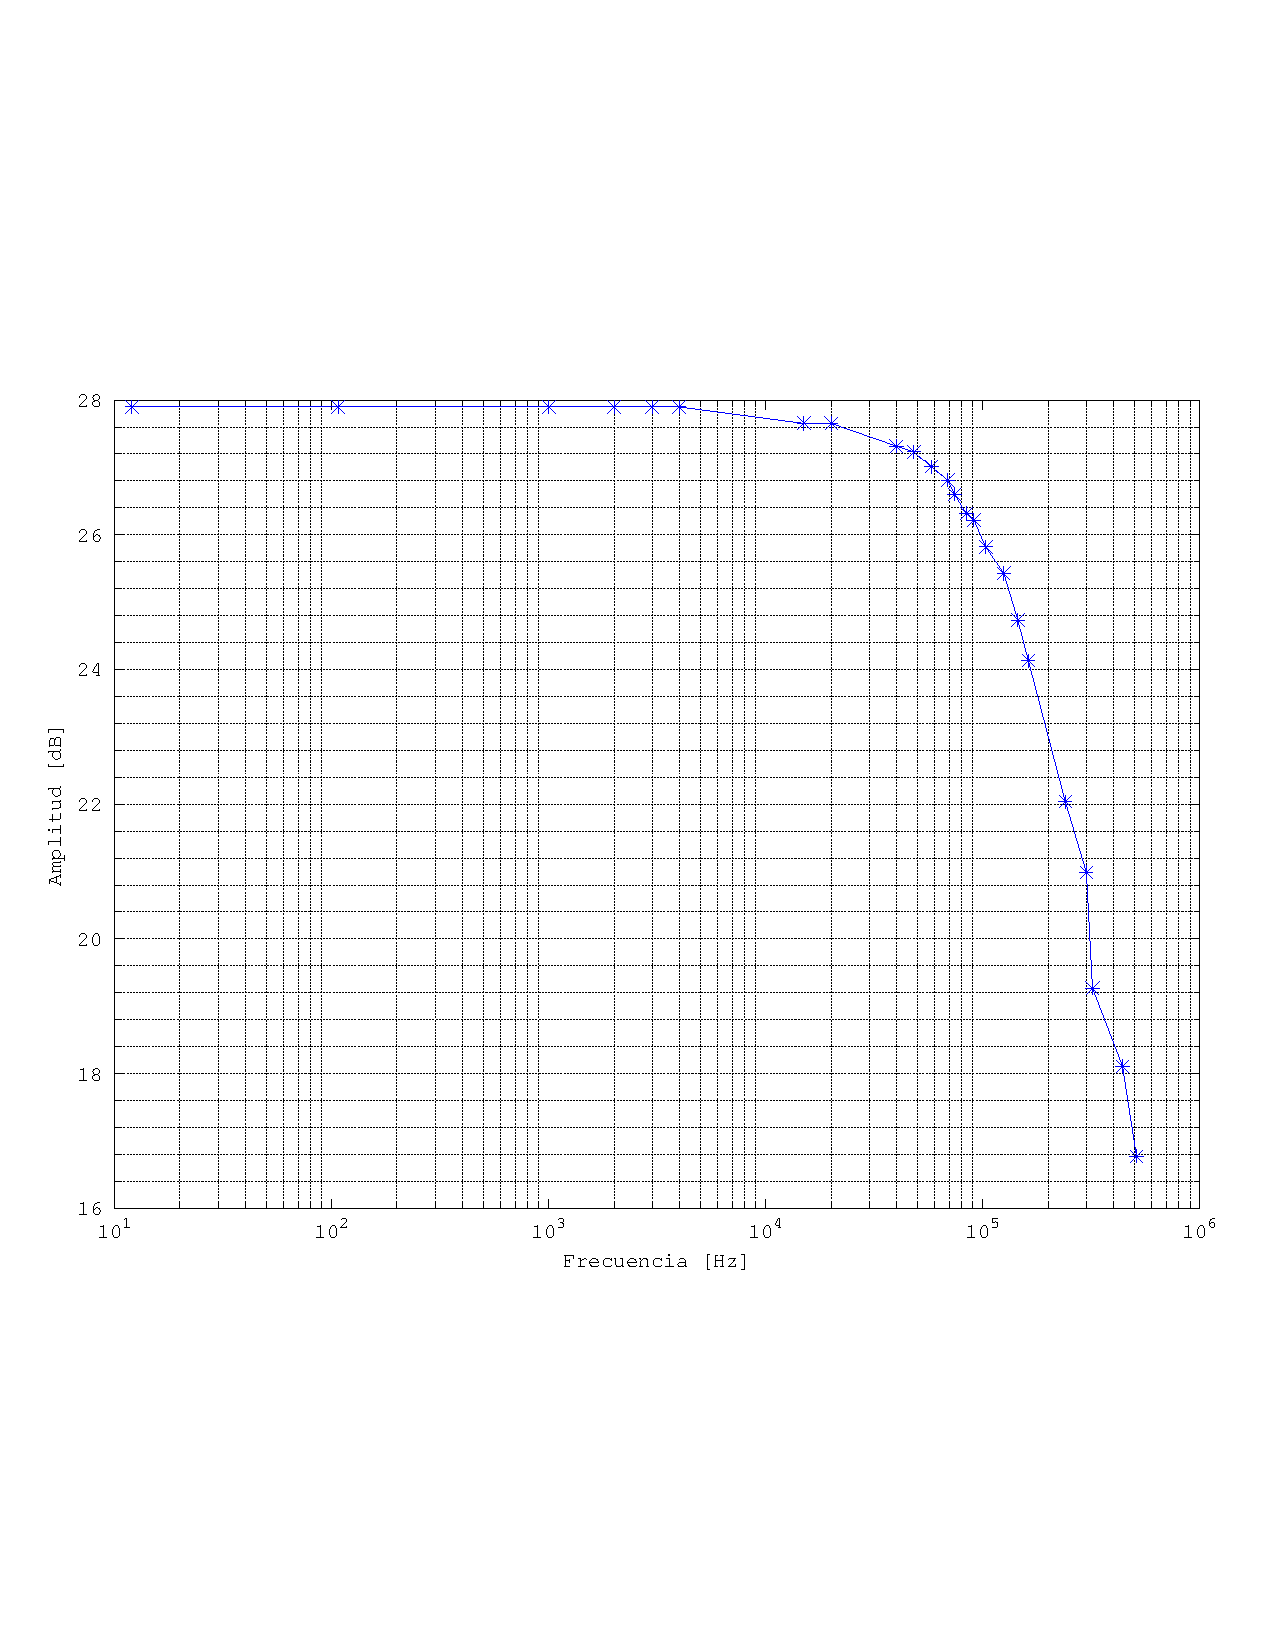
\includegraphics[scale=0.5]{./Figuras/bw_total.pdf}
			\caption{Respuesta en frecuencia a 1W.}
		\end{figure}

		\subsubsection{Relación Señal a Ruido}
		Para realizar la medición de la SNR se utilizó el programa Spectra Plus en el cual se midio con ruido blanco para geerar el piso que presenta la placa de sonido y luego se generó una señal a $1KHz$ y $1W$ midiendo la salida con el banco de medición de la Figura \ref{fig:thd_bco} .



			\begin{figure}[H]
				\centering
				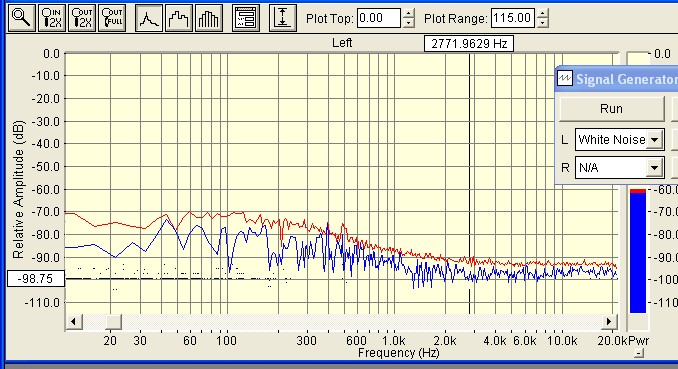
\includegraphics[scale=0.6]{./Figuras/ruido_balnco.jpg}
			\caption{Piso de ruido.}
			\end{figure}

			\begin{figure}[H]
				\centering
				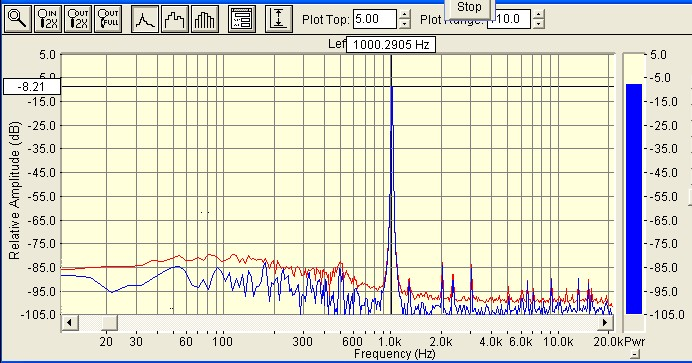
\includegraphics[scale=0.6]{./Figuras/SNR_1K_1W_imagen2.jpg}
			\caption{Salida a 1 W y 1 Khz.}
			\end{figure}


			Calculando:

			\begin{equation*}
			SNR_{db}  = 20 \dot log(\frac{V_{ruido}}{V_o}) = V_{ruido_{dB}} - V_{o_{dB}}
			\end{equation*}

			Por lo tanto: 

			\begin{equation*}
			SNR_{db}  = 98.75 - 8.21 = 90.54 dB  
			\end{equation*}


%		
%		\subsubsection{Rechazo de Ruido de la Fuente de Alimentación}
%
%		\subsubsection{Máxima eficiencia del amplificador}
%
%		\subsubsection{Comportamiento térmico}
